Given, the system of equations in matrix equation format are as below
\begin{align}
\myvec{2 & 3\\2 & -4\\m & -1}
\vec{x}=
\myvec{11\\-24\\-3}
\end{align}
\textbf{Step1}: Assuming the system of equations are consistent, lets reduce the  augmented matrix [A'b], to find the value of m.
\begin{align}
\begin{split}
\myvec{2 & 3 & 11\\2 & -4 & -24\\m & -1 & -3}\\
\xleftrightarrow[]{R_2 \leftarrow {R_2-R_1}}\\
\myvec{2 & 3 & 11\\0 & -7 & -35\\m & -1 & -3}\\
\xleftrightarrow []{R_3\leftarrow {2R_3+R_1}}\\
\myvec{2 & 3 & 11\\0 & -7 & -35\\2m+2 & 1 & 5}\\
\xleftrightarrow []{R_3\leftarrow {R_2+7R_3}}\\
\myvec{2 & 3 & 11\\0 & -7 & -35\\14m+14 & 0 & 0}
\end{split}
\end{align}
Since the system of equations are assumed consistent,
\begin{equation}\label{eq:solutions/line_plane/17finaleq}
\begin{split}
\Rightarrow 14m+14 = 0\\
\Rightarrow m=-1
\end{split}
\end{equation}
\textbf{Step2}:The system of equations can be represented as vectors as below:
\begin{figure}
  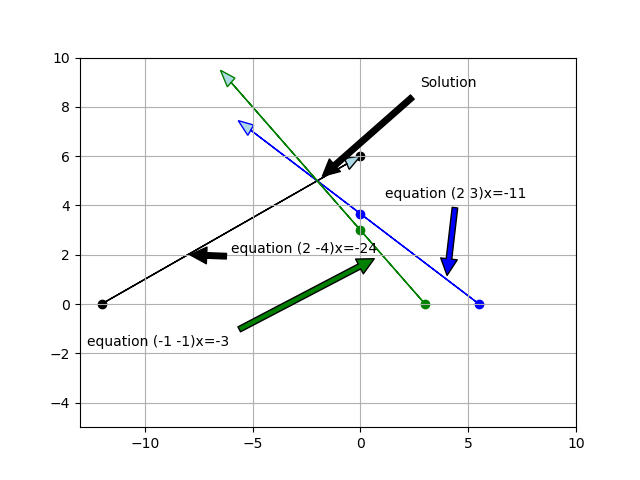
\includegraphics[width=\linewidth]{./solutions/line_plane/17/assignment1solution_graph1.png}
  \caption{System of Equations displaying intersecting at a point (-2 5).}
  \label{eq:solutions/line_plane/17fig:graph1}
\end{figure}
\\
\begin{figure}
	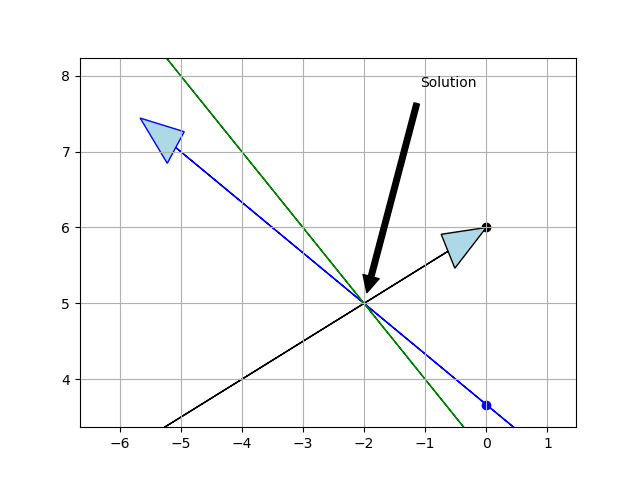
\includegraphics[width=\linewidth]{./solutions/line_plane/17/assignment1solution_graph.png}
  \caption{A zoomed in view of System of Equations displaying intersecting at a point (-2 5).}
  \label{eq:solutions/line_plane/17fig:graph2}
\end{figure}
